\documentclass[a4paper, fontsize=11pt]{article}
\usepackage[english, ngerman]{babel}
\usepackage[autostyle]{csquotes}
\usepackage{natbib}

% \bibliographystyle{ksfh_nat}
% \bibliographystyle{apa}
\bibliographystyle{apalike}
% \bibliographystyle{plainnat}

\usepackage{hyperref}
\usepackage{graphicx}
\usepackage{titlesec}
\usepackage{subcaption}
% \usepackage[raggedrightboxes]{ragged2e}
% \usepackage{pgf-pie}
% \usepackage{pgfplots}
\usepackage[acronym, toc, numberedsection]{glossaries}

\usepackage{hyphenat}
% \hyphenation{Mathe-matik wieder-gewinnen}
\usepackage[T1]{fontenc}

\makenoidxglossaries
\newacronym{dom}{DOM}{Document Object Model}
\newacronym{html}{HTML}{Hypertext Markup Language}
\newacronym{css}{CSS}{Cascading Style Sheet}
\newacronym{js}{JS}{JavaScript}
\newacronym{csr}{CSR}{Client-side Rendering}
\newacronym{ssr}{SSR}{Server-side Rendering}
\newacronym{svg}{SVG}{Support Vector Graphic}

\title{WIP: Mega-fast or just super-fast? Performance differences of mainstream JavaScript frameworks for web application}
\author{Andreas Nicklaus}

\makeatletter
\let\Title\@title
\let\Author\@author

\makeatother

\begin{document}

\begin{titlepage}
	
  \begin{center}

    
\includegraphics[width=150px, keepaspectratio]{img/hdm-logo.png}
    
    \vspace{30px}
    {\large Masterarbeit im Studiengang Computer Science and Media}
    
    \vspace{20px}
    {\LARGE \Title}
    
    \vspace{20px}
    \noindent\rule{\textwidth}{1pt}
    
    \vspace{15px}
    vorgelegt von
    
    \vspace{10px}
    \textbf{{\large \Author}}
    
    % \vspace{5px}
    Matrikelnummer 44835
    
    \vspace{10px}
    an der Hochschule der Medien Stuttgart
    
    \vspace{10px}
    am \today
    
    \vspace{10px}
    zur Erlangung des akademischen Grades eines Master of Science
  \end{center}	
  
  \vfill
  
  \begin{tabular}[t]{ll}
    Erst-Prüfer: & Prof. Dr. Fridtjof Toenniessen \\
    Zweit-Prüfer: & Stephan Soller
  \end{tabular}		
\end{titlepage}

\selectlanguage{ngerman}

\section*{Ehrenwörtliche Erklärung}
	
	Hiermit versichere ich, \Author, ehrenwörtlich, dass ich die
	vorliegende Masterarbeit mit dem Titel: „\Title“ selbstständig und ohne fremde Hilfe verfasst und keine
	anderen als die angegebenen Hilfsmittel benutzt habe. Die Stellen der Arbeit, die dem
	Wortlaut oder dem Sinn nach anderen Werken entnommen wurden, sind in jedem Fall
	unter Angabe der Quelle kenntlich gemacht. Die Arbeit ist noch nicht veröffentlicht oder
	in anderer Form als Prüfungsleistung vorgelegt worden.\\
	
	Ich habe die Bedeutung der ehrenwörtlichen Versicherung und die prüfungsrechtlichen
	Folgen (§26 Abs. 2 Bachelor-SPO (6 Semester), § 24 Abs. 2 Bachelor-SPO (7 Semester), §
	23 Abs. 2 Master-SPO (3 Semester) bzw. § 19 Abs. 2 Master-SPO (4 Semester und
	berufsbegleitend) der HdM) einer unrichtigen oder unvollständigen ehrenwörtlichen
	Versicherung zur Kenntnis genommen.
	\vspace{30px}
	
	Eislingen, den \today
	\vspace{20px}
	
	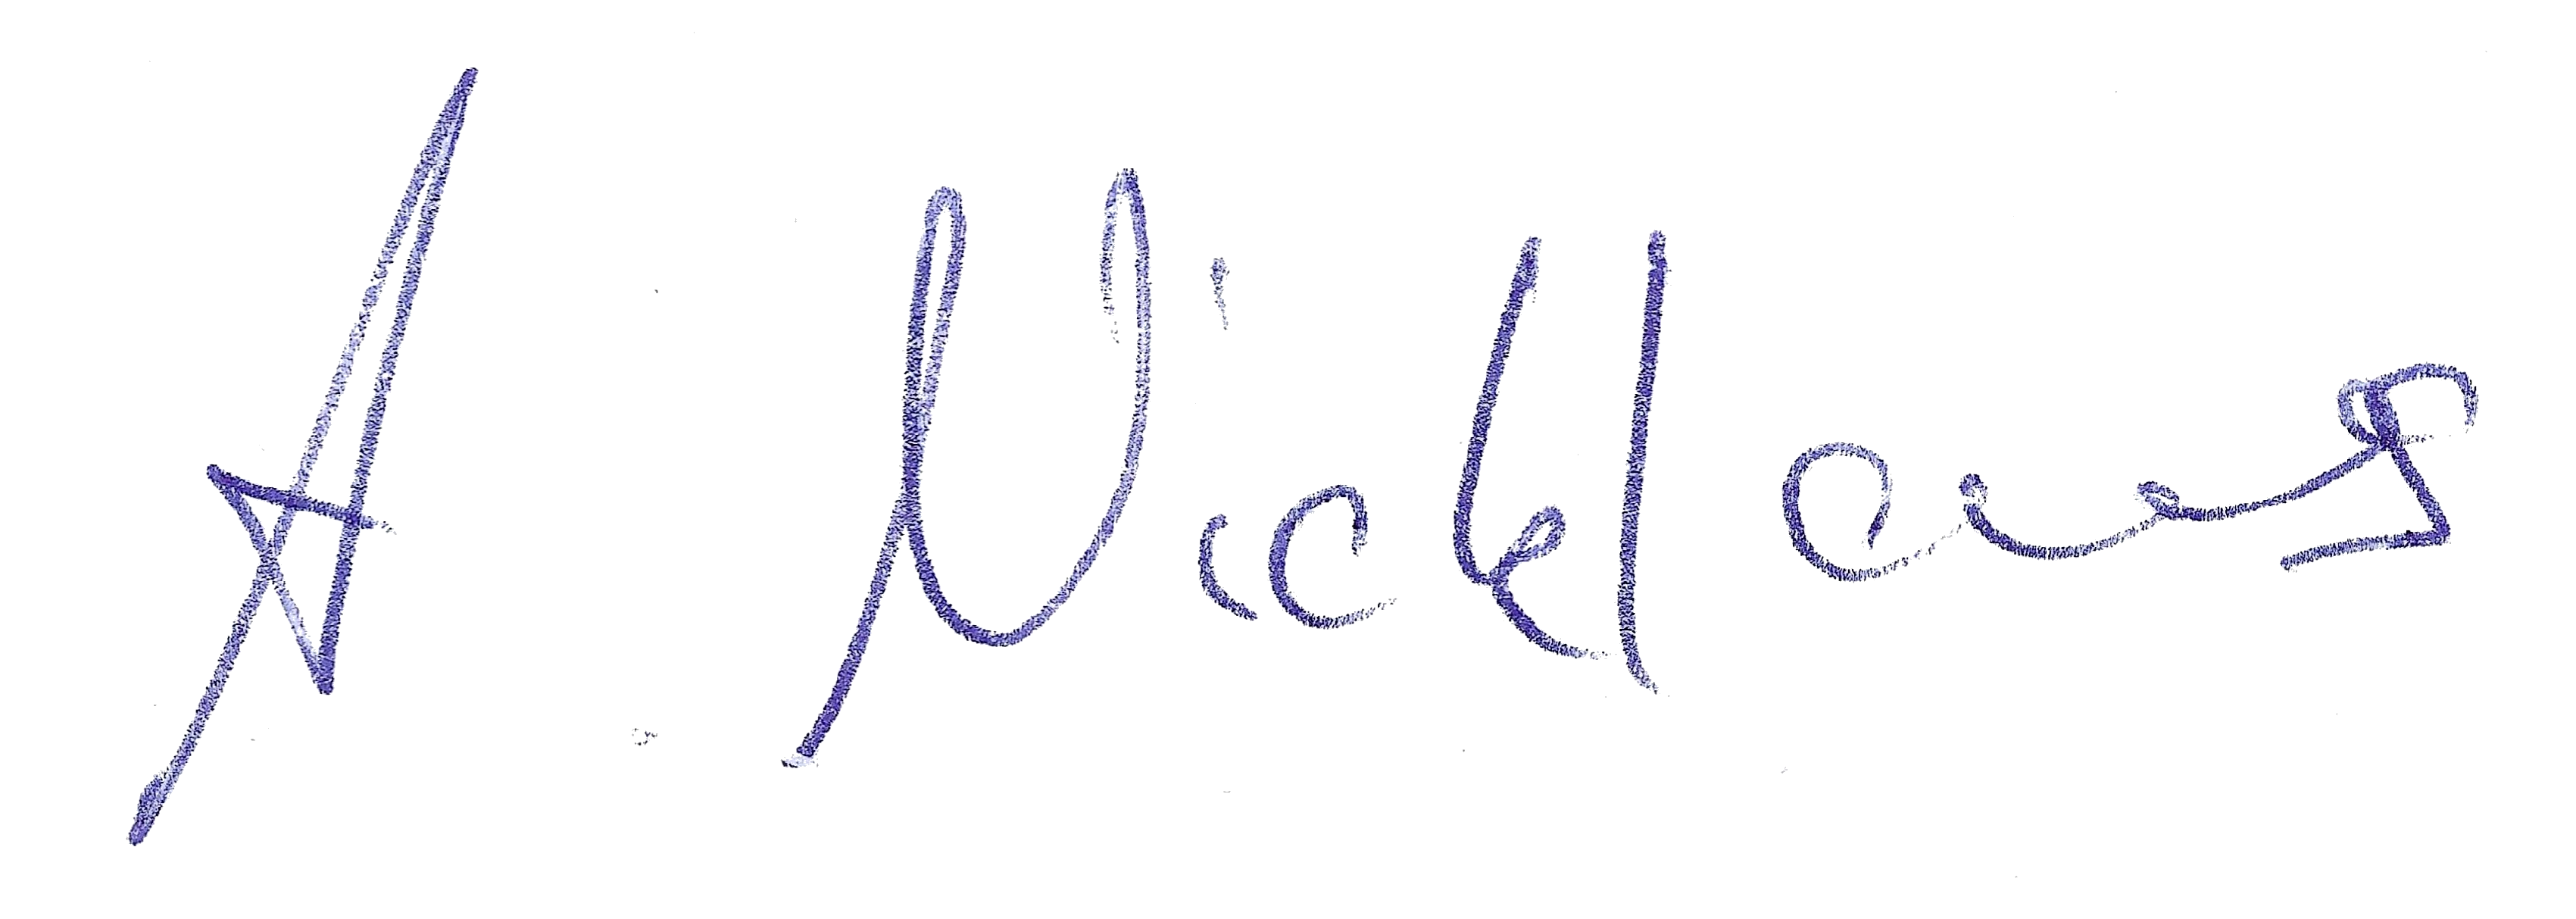
\includegraphics[height=60px]{img/unterschrift.png}
%	\vspace{60px}
	\vspace{10px}
	
	\Author

\pagebreak

\selectlanguage{ngerman}
\begin{abstract}
  Diese Arbeit kurz und knackig.
  % TODO
\end{abstract}

\selectlanguage{english}
\begin{abstract}
  This work in a nutshell.
  % TODO
\end{abstract}

\vfill

\noindent\textbf{Dislaimer:} This paper has been written with the help of AI tools for translating sources and outlining parts of the written content.
All content has been written or created by the author unless marked otherwise.

\pagebreak

\tableofcontents
\pagebreak

\section{Introduction}\label{sec:introduction}
Throughout the evolution of the world wide web, many changes have disrupted the way websites are created.
From simple file servers run by few selected institutions, simple static web pages and dynamic services like blogs and forums to websites created with the help UI tools and web development frameworks, mainly written in JavaScript, development has changed drastically since its beginning.

Older web pages often lacked features, that developers today work with as a matter of course.
Yet their load and rendering most likely would be brazingly fast with today's technological advancements in networking, browser functionalities and user equipment.
Modern websites though are often bigger in size, have a lot more features and are in many respects more complex.
Due to the increased complexity, the mere volume of a webiste's data has increased, especially with more and more multimedia files
That in return has increased the demand for better performance on all components of the load and rendering process.
This technological advancement has upped the technological sophistication for development tools as well.
Today's modern web development frameworks support developers with tools to create sites and applications through terminal commands.
They often increase the content-per-line-of-code quota through implicit page generation in contrast to the explicit writing of source code from earlier times.
Many frameworks even feature configuration options for directly hosting the webpage.

As the generation process changed from writing code manually to automatically, this implicit page generation undoubtedly increased speed through faster content generation and a greater developer experience for some developers.
Because developer experience varies between different frameworks and some approaches are more intuitive to respective developers, a current trend has evolved for developers to become experts in a single framework rather than many.
This trend leads to a tribal conflict as to which framework is better than others with each tribe being convinced that their framework is the best.
There is no apparant way to determine a \enquote{best framework} in terms of Developer Experience because it is a subjective criterion.
The performance of a framework as assessed by the developer can be similar or greatly different, depending on the frameworks and the interviewees.

When it comes to User Experience and especially the Perceived User Experience however, there are plentiful collections of metrics and criteria to choose from so as to determine the performance of websites, not frameworks.
The optimization of websites has become a goal during development because it has a real effect on both the ranking of web pages in search engines and the user behavior.
Both effects create business interests and financial incentives to invest resources into performance optimization.
However, the lack of research on the topic suggests either a consensus for a negligible effect of the development framework on the website's performance or a lack of knowledge of the effect.
Measurements on the effect of the development framework are a major convoluted task simply because the performance of a specific website can be dependent on many other factors such as the user's device, browser, networking hardware or server-side hardware.
The number of possible combinations of factors and their reliability makes it difficult to measure a single performance run with a reliable result.
Every single result is only a small part of a large number of possible performances the same application could achieve with different parameters.
It is therefore perceivable that a \enquote{perfect combination} of hard- and software exists for each framework or in general, but it is currently not possible to find such a combination because the necessary data is missing.

Many modern web tracking services provide data about the user, the user's devices, current page load times and so on.
This data is helpful in determining current poor performances and therefore possible starting points for optimization efforts.
But it gives very little information about recommended actions or recommended choice of framework for a redesign of a web application.
Relying on marketing material for choice of framework is equally questionable because most modern frameworks claim to be fast, easy to use and performance efficient.
This suggests that each would be a great choice for developers.

In order to find a suitable framework for an application, a set of metrics needs to be at least outlined for comparison.
Many former studies suggest metrics to be relevant for the User Experience or Search Engine Optimization.
Content metrics such as word count or presence of meta tags might be important for some performance measurements, but might also have no effect on the User Experience.
In contrast, rendering metrics such as page load time or page weight might be ascribed to the framework used during development.

The performance of a framework towards the user can very rarely be compared because there are no publicly available comparisons between exact replicas of web applications built with different frameworks.
Therefore, a comparative study between the same website built with different frameworks is needed to get as close as possible to an exact website replica.
With this data, an informed choice might be made for other projects.

The goals of this paper are to propose a set of metrics that allow comparing mainstream JavaScript frameworks for web applications, to provide a comparative study between selected frameworks and create a tool to compare the rendering performance of a page as a whole and of dynamic components within a page.

\section{Related Work}\label{sec:relatedwork}
\section{Design}\label{sec:design}

Whereas the following chapters cover the implementation of testing and evaluation of results, this section introduces concept of the comparative study.
The goals of and requirements for the example application, the differences and choices for the hosting environments for testing and the tools for testing as well as selected metrics will be described here.

\subsection{Example Application}\label{subsec:exampleapplication}
% What goals does should the example app fulfil?
% What parts does the example app consist of?
% What requirements does the app cover?
%
% 1. App Idea
% 2. Pages
% 3. Page intention & type
% 4. Multimedia Files & Video Autoplay
% 
% MOSCOW-Analyse
% UML-Diagramme: Services, Pages, Entities

The example application for the study is designed to be a benchmark application for testing.
The following goals were considered during the design process:

\begin{enumerate}
  \item \textbf{Page types}: With the goal of covering most kinds of webpages, three types were identified based on the time of data loading.\label{enum:pagetypes}
  These types differ in timing at which the \acrshort{dom} content is loaded or updated.
  The definition of a finished load or update for this work is that the linking of resources does constitute a finished load or update of the webpage regardless of the load time of said resource.
  The only condition for that is that any linked resources do not update the \acrshort{dom} in any way.
  If a resources does, then the load or update is considered not finished.
  % TODO: WOW! Ändere die obere Definition noch mal
  \begin{enumerate}
    \item Static Pages are webpages which do not change their content after the initial response from the web server.
    The initial \acrshort{html} document already contains the data that is necessary to create a complete \acrshort{dom}.
    \item Delayed Pages do not have a complete \acrshort{dom} after loading and parsing of the initial \acrshort{html} document.
    Some data or content is loaded and inserted (or removed) into the \acrshort{dom} after the initial render.
    The time of these updates can be any time after the initial render, but the execution of code or start of request for the resource that is responsible for the update has to be directly or indirecly triggered by the content of the initial \acrshort{dom} or \acrshort{html} document.
    \item Dynamic Pages can be updated or update themselves by events that are not triggered by the content of the initial \acrshort{dom} or \acrshort{html} document.
    These events can either be triggered by user interaction or other events such as websocket messages.
    The time of such updates is by their nature not predictable.
    Dynamic pages are either static or delayed with additional possibilities for updates.
  \end{enumerate}
  This list is created with the knowledge that frameworks or other technology such as caching may move a webpage from one type to another.

  \item \textbf{Modern Development Practices}: The example application should contain modern development practices that do project onto the \acrshort{dom}.
  Practices that have no effect on either the projection of data or user interaction, such as coding styles or project management, are considered to have no effect the performance of the page.
  
  \begin{enumerate}
    \item Components: All pages of the app have to consist of components that encapsulate reproducable \acrshort{html} snippets and may project data onto the \acrshort{dom}.
    \item List iteration: Because iterating long lists may decrease performance noticably, some components or pages should implement list iteration.
    \item String interpolation: Although it is not considered a performance issue before testing, string interpolation is prevalent in all modern frameworks known to the author.
    \item Services: \label{enum:services} Separation of functions in services is wide spread practice to reduce code duplicates and easy refactoring.
    In this case, services also allow to intentionaly implement delays for testing purposes.
  \end{enumerate}
  
  \item \textbf{\acrshort{css}}: Even though the usage of \acrshort{css} can in no way be considered a modern practice, it is still used on effectively every webpage.
  Additionally, stylesheets are considered a render-blocking resource that impacts performance negatively. % TODO: source for render-blocking resource
  For this purpose, \acrshort{css} shall be implemented for both pages and components.
  
  \item \textbf{Rendering time}: In addition to page type depending on the time of data load, the machine and time of composing the \acrshort{dom} is dependent on the content availability.
  For this paper, three different types are considered:
  \begin{enumerate}
    \item \acrfull{csr}: The initial request gets a response with a mostly empty \acrshort{html} document (\enquote{sceleton}) except linked \acrshort{css} and \acrshort{js} resources which after loading, parsing and execution update the \acrshort{dom}.
    \item \acrfull{ssr}: Updates that happened after receiving the sceleton through \acrshort{js} code execution on \acrshort{csr}, happens before the initial request is responded to on the web server.
    The initial \acrshort{html} document is filled and no longer a skeleton with \acrshort{ssr}.
    Therefore, it has greater byte size.
    \acrlong{ssr} requires an \enquote{active} frontend server rather than only a file server to execute code.
    \item Prerendering: Rendering happens during build time of the application.
    This increases the build time and the byte size of the initial \acrshort{html} document, but only a file server is needed for hosting.
  \end{enumerate}

  \item \textbf{Multimedia}: Most of network load and therefore network delay is made up by multimedia files.
  Although compression has gotten better over time, the byte size made up by multimedia files of a webpage has gotten larger over the last years. % TODO: source
  Therefore, size optimization of image and video files is considered a major part of performance optimization and a great potential for a performance increase by the used framework.

\end{enumerate}

Based on these considerations, the application \enquote{NotInstagram} was designed as a comparable example application.
It is heavily inspired by Instagram and a partial reproduction of its app design. % TODO: source to IG
\enquote{NotInstagram} consists of four pages (see figure \ref{fig:screenshots}).
\ref{subfig:index} shows the design of the Feed page.
It is the start page of the app and contains 4 parts: the header, the profile list, the post list and a footer.
Each item of the feed page is to be implemented as its own component or components.
The plus icon in the header links to the create page, the footer links to the about page and every instance of a profile picture and profile name links to the profile page.
The later contains profile information including a profile picture, name, user handle / ID, profile creation time, caption and a grid of all the user's posts (see figure \ref{subfig:user}).
The profile component encapsulates all HTML elements of that page except the header containing the app logo and X icon, which both link back to the feed page.
Both the feed page and the profile page are generally expected to classify as delayed pages, because the content of profile and posts lists can only be loaded after the page load.

The Create page (see figure \ref{subfig:create}) has three parts.
The header contains the app's logo and a X icon linking to the feed.
A form with three \verb|<input>| elements and a \verb|<button>| element allows the input of an multimedia source (image or video) and a text caption.
The multimedia source can either be an URL or a selection from a list of preuploaded files.
The post caption is a pure text input.
The lower part of the page is the post preview, in which some predefined information such as user profile and the user inputs are combined.
As such, the profile page is a static page until the user uses the creation form, at which point is has to be considered a dynamic page.
The About page (see figure \ref{subfig:about}) is designed to statically display information about the application.
It is a static page because no content is loaded after a delay and no user inputs are possible.

With these pages all \hyperref[enum:pagetypes]{page types} are covered for testing.
The about page and create page are static, whereas the feed page and profile page are partly static (header and footer), but mostly delayed.
The create page is the only page with dynamic content.

\begin{figure}[ht!]
  \begin{subfigure}{0.49\linewidth}
    \begin{center}
      
\includegraphics[width=\linewidth, height=0.3\textheight, keepaspectratio]{img/ig-clone/Feed.png}
      % TODO: Plus-Icon im Screenshot fehlt
    \end{center}
    \caption{Feed / Index Page (/)}\label{subfig:index}
  \end{subfigure}
  \begin{subfigure}{0.49\linewidth}
    \begin{center}
      
\includegraphics[width=\linewidth, height=0.3\textheight, keepaspectratio]{img/ig-clone/Informationsseite.png}
      % TODO: Profilseite
    \end{center}
    \caption{Profile Page (/user/@PeterPoster)}\label{subfig:user}
  \end{subfigure}
  \begin{subfigure}{0.49\linewidth}
    \begin{center}
      
\includegraphics[width=\linewidth, height=0.3\textheight, keepaspectratio]{img/ig-clone/Beitrag erstellen.png}
      % TODO: X-Icon fehlt
    \end{center}
    \caption{Create Page (/create)}\label{subfig:create}
  \end{subfigure}
  \begin{subfigure}{0.49\linewidth}
    \begin{center}
      
\includegraphics[width=\linewidth, height=0.3\textheight, keepaspectratio]{img/ig-clone/Informationsseite.png}
      % TODO: Backlink fehlt
    \end{center}
    \caption{About Page (/about)}\label{subfig:about}
  \end{subfigure}
  \caption{Screenshots of the NotInstagram application's pages (path in parentheses)}\label{fig:screenshots}
\end{figure}

The data fetching / loading is designed to be implemented \hyperref[enum:services]{services}.
For NotInstagram two different services are needed.
The PostService is a service for all components to query posts.
The method \verb|getAll()| returns a list of all posts by all users and \verb|getByUserHandle(handle)| returns the same list filtered by those posted by a user with the handle equal to the function parameter.
ProfileService is a service to query user profiles.
It has the same two methods which return all user profiles and only one user profile respectively.
Services are designed asynchronous, but the data is not queried from a server external to the browser, but hard coded.
This design decision is based on the premise that delay can be coded into or out of asynchronous functions to mimic network delay for testing purposes if necessary.

Figure \ref{fig:uml} describes the usage of components and services within page views.
It displays the four pages of NotInstagram as views, the two services and 15 components.
Seven of those components are icon components.
Those components serve as wrappers for \acrshort{svg}s to ensure their correct scale and style.
\verb|XIcon| poses an exception to the design as it a wrapper for a \verb|PlusIcon| component rotated by 45°.
The colored arrows show the usage of one of the services.
Both \verb|FeedView| and \verb|ProfileView| use both services to load data.
For the Feed page, both \verb|PostService.getAll()| and \verb|ProfileServices.getAll()| are needed to pass the data to \verb|PostList| and \verb|ProfileList|.
Notably, each \verb|Post| component accesses the ProfileService again, to get the profile image and name for its headline, even if the information is available in a parent or grandparent component.
Figure \ref{fig:classes} displays the connections between post and profile object instances.
The member \verb|userhandle| of a post references the member \verb|handle| of a user profile.
The Profile page needs access to the service to get the information of the requested profile and a list of posts from the \verb|getByUserHandle| methods to pass into the \verb|Profile| component.
\verb|LogoHeader|, \verb|NotInstagramLogo| and \verb|InfoBlock| are not data-presenting components, but rather styling components.
Their only function is styling text or projecting \acrshort{html} elements with \acrshort{css} information.

\begin{figure}
  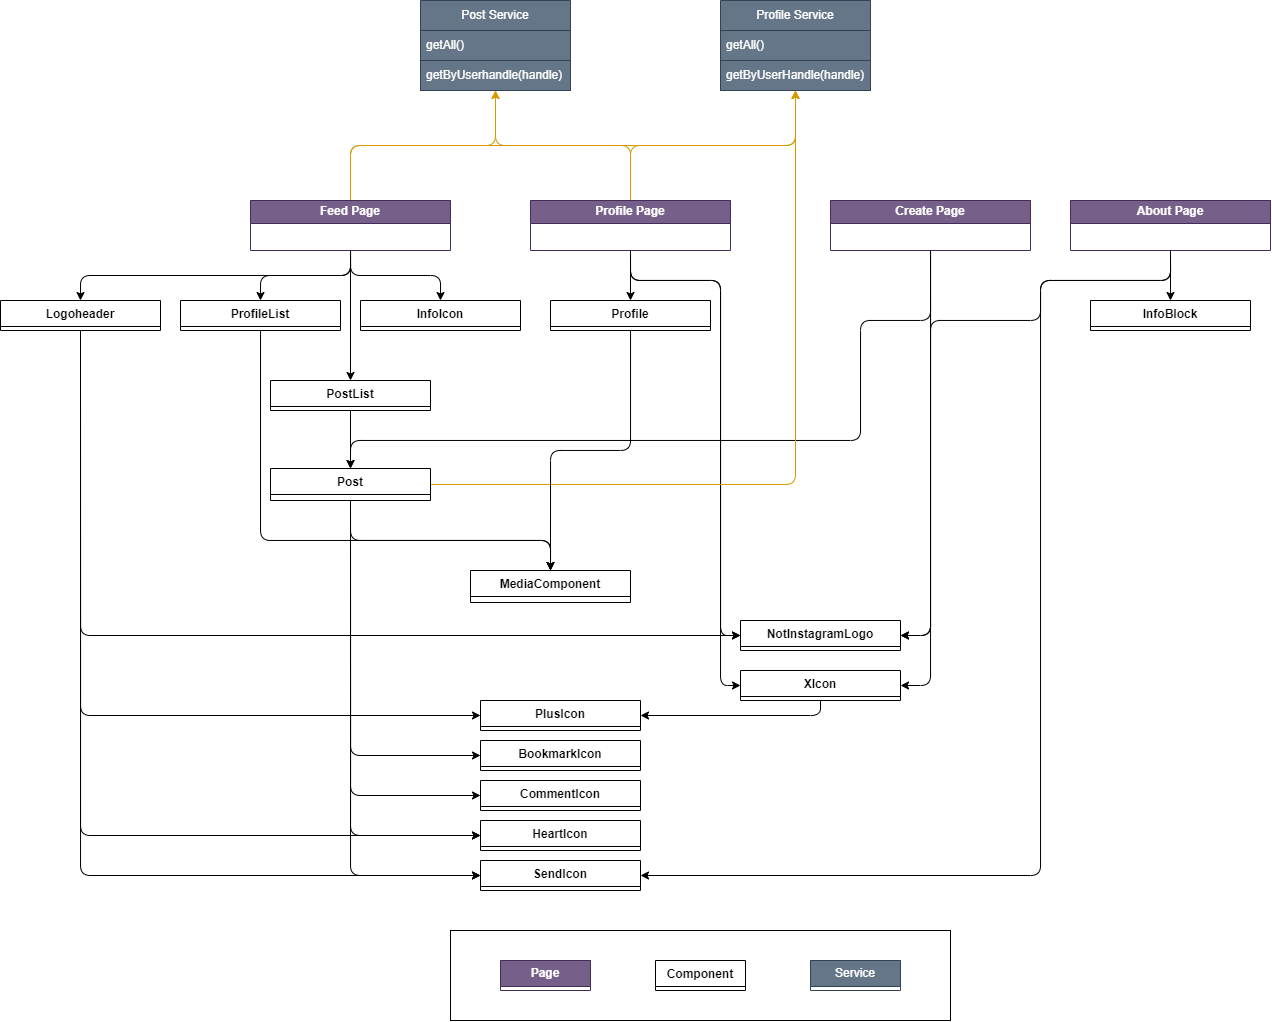
\includegraphics[width=\linewidth]{diagrams/uml.png}
  % TODO: LogoHeader references NotInstagramLogo
  \caption{Pages, Components ands Services of the NotInstagram application}\label{fig:uml}
\end{figure}
\begin{figure}
  \begin{center}
    
\includegraphics[width=0.5\linewidth]{diagrams/entities.png}
  \end{center}
  \caption{Classes used by the NotInstagram services}\label{fig:classes}
\end{figure}

In contrast, the \verb|MediaComponent| is designed as a way to allow both internal and external images and video source.
It is used by \verb|ProfileList|, \verb|Post| and \verb|Profile| to display posts and profile images.
It's main goals is to decide based on the passed image source string how to project the multimedia file onto the \acrshort{dom}.
The component accepts source strings for images and videos, differentiated against by the string's ending and therefore the file's extension.
If it is a local image, namely an image that was available for optimization at build time, the best available form of optimized \verb|<img>| tag should be used.
For external image links starting with \enquote{http://} or \enquote{https://} a less optimized or unoptimized \verb|<img>| tag shall be inserted into the \acrshort{dom}.
For videos, any source string is to be projected onto a \verb|<source>| tag with identical \verb|<video>| wrapper.

The application referres to local images, which can possibly be optimized, and external images, which cannot be optimized.
The reason for this is the assumption made for this project that optimizing multimedia files uploaded by a user and referencing them in a matter suitable for this application is not suitable for this work.
Rather the better alternative for serving the use case of the application would be a dedicated server for encoding, decoding and generally optimizing multimedia files.
Since this solution would be independent from the frontend framework's performance, a distinction is only made between static images, called local images here, with and external images with full URLs.

\subsection{Hosting Environments}\label{subsec:hostingenvironments}
% Based on former work, networking plays a vital role in performance and load times
% 
% What exactly should be tested?
% What requirements do the environments have to cover?
% What properties should be considered for the environments?
% TODO: what are the most used hosting environments?
% 
% 1. Vercel
%    1. Reason
%    2. Problems
%    3. Solutions
% 2. Local
%    1. Reason (Network delay)
%    2. Problems


\subsection{Testing Tools}\label{subsec:testingtools}
% What tools were using testing and how do they work? 
% What requirements should be fulfilled by the tools
% 
% 1. Introduction into Playwright
% 2. Introduction into Lighthouse CLI
% 
% What problems are expected to arise from these tools?
% What requirements are covered by which tool?

\subsubsection{Performance Metrics}
% What metrics can be measured?
% What metrics should be used?
% What metrics will be used?
% 
% 1. Lighthouse performance
% 2. Page weight
% 3. Largest/First Contentful/Meaningful Paint
% 4. TTFB/TTI/SpeedIndex

\subsubsection{Component Load Times}
% Measuring JS-dependent parts of the webpage
% 
% 1. Dom Updates with MutationObserver
% 2. Problems with MutationObservers and Playwright

\subsubsection{Component Update Times}
% 3rd type of update through JS
% 
% - Interesting comparisons with reasoning and expectation
%   - MPA vs SPA
%   - Angular vs React vs Vue
%   - Nuxt vs Vue und Next vs React
%   - Vue-basiert vs React-basiert
%   - Svelte vs Astro
% - Page Load Times

\section{Implementation}\label{sec:implementation}
\subsection{Components}\label{subsec:components}
% Notable components and HTML elements
% How are they constructed?
% How are they projected onto the DOM?
% 
% 1. MediaComponent
% 2. About Aufbau
% 3. Post mit und ohne Daten
% 4. Astro CreateForm
\subsection{Tests}\label{subsec:tests}
% How are tests configured and implemented?
% What is measured, stored and evaluated?
% 
% - Test categories
%   - Page Load
%   - Dynamic Component Load Times
%   - State Change Times
% - Playwright test configuration
% - Browser Choices: Reasoning and test implementation

\section{Evaluation}\label{sec:evaluation}
\subsection{Page Load Times}\label{subsec:pageloadtimes}
% 1. Which pages load fast?
% 2. How much does much post-rendering-data add to load time?
% 3. Which frameworks creates fast-loading pages?
% 4. Does it match my expectations?

\subsection{Component Load Times}\label{subsec:componentloadtimes}
% 1. Which components load with delay?
% 2. Which frameworks have fast-loading delayed components?
% 3. Do pre-rendered pages even have delayed components?

\subsection{Component Update Times}\label{subsec:componentupdatetimes}
% 1. Which differences can be made out towards [Component update times](#component-update-times)?
% 2. Which HTML-Elements even update?
% 3. Which frameworks update HTML-Elements faster than others?

\section{Conclusion}\label{sec:conclusion}
% 1. Which framework works best with page load times?
% 2. Which framework works best with component load times?
% 3. Which framework works best with component update times?

\section{Summary}\label{sec:summary}

\pagebreak

\appendix
\glsaddall
\printnoidxglossary[type=\acronymtype,nonumberlist,style=long]

% \cite{5GEfficiencyOverview}

\nocite{*}
\bibliography{sources}{}
\end{document}